\documentclass[11pt]{article}

\usepackage[T1]{fontenc}
\usepackage{lmodern}
\usepackage[margin=1in]{geometry}
\usepackage{microtype}
\usepackage{amsmath,amssymb,amsthm}
\usepackage{booktabs}
\usepackage{graphicx}
\usepackage{xcolor}
\usepackage[font=small,labelfont=bf]{caption}
\usepackage[numbers,sort&compress]{natbib}
\usepackage[colorlinks=true,linkcolor=blue!50!black,citecolor=blue!50!black,urlcolor=blue!50!black]{hyperref}
\usepackage[capitalise,noabbrev]{cleveref}

\graphicspath{{figures/}}
\setlength{\parskip}{3pt}
\setlength{\tabcolsep}{4.5pt}
\setlength{\textfloatsep}{12pt plus 2pt minus 4pt}
\setlength{\floatsep}{10pt plus 2pt minus 2pt}
\setlength{\abovecaptionskip}{6pt}
\newtheorem{proposition}{Proposition}
\crefname{appsec}{Appendix}{Appendices}

% Generated by scripts/make_figures.py; do not edit.
\newcommand{\btCachedNet}{$-$\$192k}
\newcommand{\btCachedP}{0.09}
\newcommand{\btCachedSold}{59\%}
\newcommand{\btExcess}{$+$\$59k}
\newcommand{\btNet}{$+$\$292k}
\newcommand{\btP}{0.31}
\newcommand{\btPlacebo}{$+$\$233k}
\newcommand{\btRepTrades}{3}
\newcommand{\btSameExcess}{$+$\$320k}
\newcommand{\btSameP}{0.02}
\newcommand{\btSharpe}{0.99}
\newcommand{\btSold}{68\%}
\newcommand{\btTrades}{1{,}482}
\newcommand{\condFitTest}{0.38}
\newcommand{\condGapNinety}{0.61}
\newcommand{\condGapSlices}{0.64}
\newcommand{\condQFour}{1.46}
\newcommand{\condQIn}{0.31}
\newcommand{\condQInMax}{0.44}
\newcommand{\condQOne}{0.73}
\newcommand{\condTimeVal}{0.06}
\newcommand{\condWingRep}{0.55}
\newcommand{\condWingTest}{0.70}
\newcommand{\fcPTwenty}{0.27}
\newcommand{\fcRwTwenty}{4.27}
\newcommand{\fcVarTwenty}{3.90}
\newcommand{\hestonTruthNinetyCond}{0.073}
\newcommand{\hestonTruthNinetyMix}{0.40}
\newcommand{\mixFitRep}{0.068}
\newcommand{\mixFitTest}{0.071}
\newcommand{\mixFitVal}{0.121}
\newcommand{\mixGapNinety}{0.155}
\newcommand{\mixGapSlices}{0.34}
\newcommand{\mixInRep}{99\%}
\newcommand{\mixInVal}{81\%}
\newcommand{\mixTimeHeston}{7.6}
\newcommand{\mixTimeVal}{33}
\newcommand{\mixTruthFresh}{0.099}
\newcommand{\mixWingRep}{0.35}
\newcommand{\mixWingTest}{0.82}
\newcommand{\mixWingVal}{1.31}
\newcommand{\multiInFresh}{96\%}
\newcommand{\multiPrecFresh}{0.996}
\newcommand{\multiRecFresh}{0.65}
\newcommand{\multiSegFresh}{66\%}
\newcommand{\multiTime}{11}
\newcommand{\multiTruthFresh}{0.045}
\newcommand{\pnnCalVal}{0.38\%}
\newcommand{\pnnTimeVal}{109}
\newcommand{\pnnWingRep}{0.32}
\newcommand{\pnnWingVal}{0.86}
\newcommand{\refitDays}{247}
\newcommand{\refitMedian}{0.69}
\newcommand{\refitTwoX}{69}
\newcommand{\refitWorstCold}{0.53}
\newcommand{\refitWorstDay}{July~7, 2023}
\newcommand{\refitWorstWarm}{0.12}
\newcommand{\revCachedDays}{144}
\newcommand{\revCachedDiffOne}{-0.23}
\newcommand{\revCachedPOne}{0.002}
\newcommand{\revDays}{67}
\newcommand{\revDiffOne}{-0.05}
\newcommand{\revMarketPOne}{0.89}
\newcommand{\revPOne}{0.72}
\newcommand{\revSegDays}{132}
\newcommand{\robAbsorbFresh}{52\%}
\newcommand{\robPrecFresh}{0.95}
\newcommand{\robRecFresh}{0.45}
\newcommand{\robSegFresh}{29\%}
\newcommand{\segAbsorbFresh}{34\%}
\newcommand{\segPrecFresh}{0.96}
\newcommand{\segRecFresh}{0.54}
\newcommand{\segSegFresh}{43\%}
\newcommand{\skewQFour}{-0.45}
\newcommand{\skewQOne}{-0.91}
\newcommand{\spxDays}{3{,}491}
\newcommand{\spxFirstYearQuotes}{570}
\newcommand{\spxValQuotes}{6{,}305}
\newcommand{\sviCalVal}{21.89\%}
\newcommand{\sviGapNinety}{0.35}
\newcommand{\sviGapSlices}{0.65}


\newcommand{\vp}{\,vp}
\newcommand{\mixfour}{\texttt{mix4}}
\newcommand{\pnn}{\texttt{pnn}}
\newcommand{\E}{\mathbb{E}}

\title{Arbitrage-Free Implied Volatility Surfaces for SPX Options:\\
Per-Day Mixtures, a Cross-Day Neural Model, and a Test for Mispricings}
\author{Zack Holt}
\date{November 2026}

\begin{document}
\maketitle

\begin{abstract}
\noindent
We fit SPX implied volatility surfaces to end-of-day option chains (2010--2023, \spxDays{} trading
days) with models that are free of static arbitrage by construction or through penalties, and test
whether quotes far from the fitted surfaces are tradable mispricings. The best surface model,
\mixfour, mixes four extended SSVI surfaces in forward-normalized price space and is arbitrage-free
for every parameter vector. It fits the 2022 validation year to \mixFitVal\vp{} with no calendar or
butterfly violations, and it stays the closest fit on the 2023 test year among the models scored
there (\mixFitTest\vp) and on a 2016--2017 replication window (\mixFitRep\vp); a penalized network extrapolates the wings better
(\pnnWingVal{} against \mixWingVal\vp) but keeps some violations. A cross-day encoder--decoder that
decodes every latent to an arbitrage-free surface wins on stationary synthetic Heston panels,
including mispricing detection (precision \multiPrecFresh, recall \multiRecFresh), but on SPX it is
limited by regime change. On SPX the default fit's objective was more than twice what the surface
can reach on \refitTwoX{} of \refitDays{} test-year days. Once those days are refitted, quotes flagged
outside the bid-ask revert no faster than unflagged ones the next day ($p=\revPOne$), and the
\btNet{} net of a delta-hedged next-day strategy is matched by placebos on unflagged contracts
(\btPlacebo; $p=\btP$ for the difference). Every setting was frozen on validation years before each
test run, and we report how often each test window was used.
\end{abstract}

\section{Introduction}
\label{sec:intro}

An implied volatility surface summarizes a day's option chain as a function $\sigma(k,T)$ of
log-moneyness and maturity. A useful surface has to interpolate between quoted strikes and
maturities, extrapolate into the wings, and be free of static arbitrage, since a surface that
admits calendar or butterfly arbitrage implies negative probabilities or prices that decrease with
maturity. A surface that is arbitrage-free and fits the quotes closely also defines a reference
price for every quote, so quotes far from it are candidate mispricings.

This report compares three ways of building such surfaces on SPX options and asks whether the
candidates they flag are tradable. The three are per-day parametric surfaces that are
arbitrage-free by theorem, per-day neural surfaces penalized towards the no-arbitrage region, and
one cross-day neural model that encodes a day's quotes into a latent vector and decodes every
latent to an arbitrage-free surface. All models are scored under one protocol on the same days,
with settings chosen on a validation year and frozen before the test years were run.

\paragraph{Findings.}
\begin{itemize}
  \item \textbf{A price-space mixture of eSSVI surfaces is the best per-day model.} Each component
  is an eSSVI surface~\citep{hendriks2019} written in coordinates in which the known sufficient
  no-arbitrage conditions become monotonicity and bound constraints, so every parameter vector is
  feasible. Four such surfaces are mixed in price space with weights that do not depend on
  maturity, which preserves the absence of arbitrage (\cref{prop:mixture}). On SPX 2022 the mixture
  fits closest (\mixFitVal\vp) with no violations on any day; it stays closest on the 2023 test year
  and on 2016--2017 (\cref{tab:models,tab:oos}).
  \item \textbf{Soft penalties extrapolate better but leave violations.} A network correcting an SSVI
  prior, with hinge penalties on a collocation grid in the spirit of~\citet{ackerer2020}, has the
  lowest held-out wing error on SPX (\pnnWingVal{} against \mixWingVal\vp{} for the mixture) and
  violates the calendar condition on \pnnCalVal{} of an extended grid.
  \item \textbf{The cross-day model is best where the regime is stationary.} On synthetic Heston
  panels it is closest to the true surface, most robust to missing strikes, and the best mispricing
  detector (\cref{tab:heston,tab:detection}). On SPX its error grows as the market leaves the
  regimes it was trained on (\cref{fig:regime}); quarterly refits close about half of that gap but
  still fit each day about five times less closely than the per-day mixture.
  \item \textbf{SPX flags are not tradable once fitting failures are removed.} The default fit of
  the mixture stops in poor local minima on some days, and a day fitted that way flags whole
  expiries. With every day refitted from the previous day's surface, flagged quotes revert no
  faster than unflagged ones at one day, their market prices move towards the model no more than
  those of unflagged quotes, and a delta-hedged strategy earns no more than matched placebos
  (\cref{sec:mispricing}). No surface model forecasts the surface better than a random walk.
\end{itemize}

\paragraph{Test-set reuse.} The test windows were used more than once, each time with every
setting frozen beforehand on the validation years (\cref{tab:windows}). The mispricing conclusion
of \cref{sec:mispricing} rests on the fourth run on SPX 2023, which was made after the fitting
failures were found and was preceded by a written prediction. We report each run, including those
whose conclusions the later runs replaced.

\paragraph{Related work.} Parametric arbitrage-free surfaces start from SVI and its surface form
SSVI, with explicit sufficient conditions for the absence of static arbitrage~\citep{gatheral2014};
eSSVI lets the correlation vary with maturity~\citep{hendriks2019}, with conditions for calibrating
and interpolating slices~\citep{corbetta2019} and a global parametrization~\citep{mingone2022}.
Nonparametric alternatives smooth prices under shape constraints~\citep{fengler2009}. Neural surfaces
either penalize the conditions on a grid~\citep{ackerer2020} or learn pricing maps for
calibration~\citep{horvath2021}. Our hard-constrained models follow the parametric line and use a
network only to generate parameters; the cross-day model borrows the set encoders and
context--target training of DeepSets~\citep{zaheer2017} and neural processes~\citep{garnelo2018}.
Surface dynamics have long been described by a few factors~\citep{cont2002}. On the trading side,
delta-hedged option positions earn the volatility risk premium~\citep{bakshi2003,carr2009}, which
is why every strategy below is compared with placebos that carry the same exposure.

\section{Data and evaluation protocol}
\label{sec:data}

\subsection{SPX option chains}

The real data are end-of-day SPX option chains from OptionsDX, 16:00\,ET snapshots for 2010--2023
(\spxDays{} trading days). For each expiry the forward $F$ and discount factor $D$ are estimated
from put--call parity, $C-P=D(F-K)$, by regressing $C-P$ on $K$ over the strikes nearest the money
(\cref{app:forwards}), so no rate or dividend data are needed. Implied volatilities are re-inverted
with Black's formula~\citep{black1976} from bid, ask and mid of out-of-the-money options. The model
coordinates are $k=\log(K/F)$, $T$ in years (ACT/365), and total implied variance
$w(k,T)=\sigma^2(k,T)\,T$. A quote is kept if it has $7\le$ DTE $\le 730$, a positive bid below the
ask, a relative spread $(a-b)/m\le 1$, $k\in[-1.5,0.75]$ and $k/(\sigma_{\text{ATM}}\sqrt{T})\in[-6,4]$,
in an expiry with at least eight such quotes. Quotes that are legs of a vertical or butterfly
arbitrage at bid and ask are flagged model-free; they are scored but never fitted.

The chains change a great deal over the sample (\cref{fig:data}). A typical day has about
\spxFirstYearQuotes{} quotes in 12--13 expiries in 2010, 2{,}400 in about 30 expiries in 2016--2017
and \spxValQuotes{} in 37 in 2022, and median half-spreads fall from about 0.75\vp{} to 0.14--0.20\vp{}
and 0.10\vp{} (0.07\vp{} in 2023). Because flags are measured in half-spreads, a fixed margin is a
larger deviation in vol points in the older windows.

\begin{figure}[t]
  \centering
  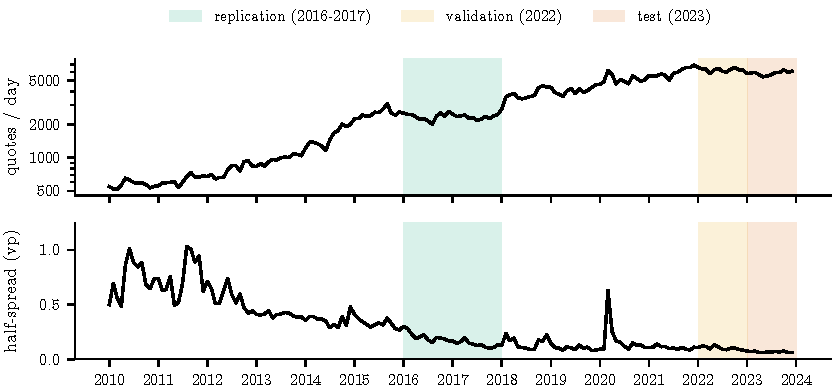
\includegraphics[width=\linewidth]{data.pdf}
  \caption{SPX chains after cleaning: monthly medians of quotes per day (log scale) and of the
  half-spread in implied vol (vol points, vp). Shading marks the evaluation windows; each conditional
  model trains only on days before the window it is scored on (\cref{tab:windows}).}
  \label{fig:data}
\end{figure}

\subsection{Synthetic panels}

Synthetic panels have a known arbitrage-free truth and labelled mispricings. Each business day
draws a variance state from a log-variance Ornstein--Uhlenbeck process correlated with spot, and
quotes Heston prices~\citep{heston1993}, computed with the COS method~\citep{fang2008}, with the
day's state as initial variance, on a realistic listing of weekly and monthly expiries. Quotes get
bid-ask spreads, noise inside the spread and tick rounding. Mispricings are injected as isolated
strikes or segments of 3--6 neighbouring strikes, shifted by 2--5 half-spreads; they persist and
decay by half each day, so a perfect detector's flags revert by $-0.50$, $-0.875$ and $-0.97$ of
their size at 1, 3 and 5 days. The main panel covers 2020--2022 (training, validation and test
year); a second panel from the same generator with a new seed (2012--2019) adds training days, and
a third (2023, a further seed) was generated for the final test and not inspected beforehand.

\subsection{Windows and protocol}

\Cref{tab:windows} lists the roles of the windows. The project was built on SPX 2018--2023;
2010--2017 was added later, for a longer training history and a second test window that no choice
was tuned on. Every setting that the test runs use was chosen on SPX 2022 or Heston 2021 and
committed before the test run.

\begin{table}[t]
  \centering\small
  \caption{Evaluation windows. A ``run'' is one evaluation of frozen settings on a test window; each
  later run was motivated by a finding and frozen on the validation years first.}
  \label{tab:windows}
  \begin{tabular}{@{}lp{5.6cm}p{6.6cm}@{}}
    \toprule
    window & role & runs on it \\
    \midrule
    SPX 2010--2021 & training of the conditional model (first 2018--2021) & -- \\
    SPX 2022 & validation: every model, penalty, detector and backtest setting & -- \\
    SPX 2023 & test & 4: mispricing tests; walk-forward refits and follow-up detectors; full-history model; mispricing tests on refitted surfaces \\
    SPX 2016--2017 & replication (conditional model retrained on 2010--2015) & 2: every model and detector; refits \\
    Heston 2020 / 2021 & training / validation & -- \\
    Heston 2022 & test & 3: detectors; follow-up detectors; refits \\
    Heston 2023 (fresh seed) & test of the nine-year conditional model & 2: follow-up detectors; refits \\
    \bottomrule
  \end{tabular}
\end{table}

Surface models are compared on blocks of two consecutive trading days every ten days (52 days of
SPX 2022, 50 of 2023 and 101 of 2016--2017). Days with heavy model-free arbitrage or poor forward
coverage are screened out. In each expiry the outer 10\% of strikes on each side are held out to
measure wing extrapolation and a random 15\% of interior strikes to measure interpolation, with the
split seeded by the date so that every model sees the same one. We report the IV RMSE in vol points
(vp) on fitted and held-out quotes, the share of model IVs inside the quoted bid-ask, and the share
of a dense $(k,T)$ grid on which the calendar or butterfly condition fails, over the quoted domain
widened by 50\% on each side. Synthetic panels also report the error against the true surface. The
mispricing tests (\cref{sec:mispricing}) use every trading day of their windows.

\section{Models}
\label{sec:models}

\subsection{Static arbitrage in total variance}

With $c(k,T)=C/(DF)$ the forward-normalized call price, a surface is free of static arbitrage if
$c$ is nondecreasing in $T$ at fixed $k$ (no calendar arbitrage) and convex and decreasing in the
strike (no butterfly or vertical arbitrage), with the usual price bounds~\citep{carr2005}. In total
variance these become~\citep{gatheral2014}
\begin{equation}
  \partial_T w(k,T) \ge 0, \qquad
  g(k) = \Bigl(1-\frac{k w'}{2w}\Bigr)^{2} - \frac{w'^{2}}{4}\Bigl(\frac{1}{w}+\frac14\Bigr)
  + \frac{w''}{2} \ge 0,
  \label{eq:conditions}
\end{equation}
where primes are derivatives in $k$ at fixed $T$: the risk-neutral density at strike $K$ is
$g(k)\,\phi(d_2)/(K\sqrt{w})$, so it is nonnegative exactly where $g$ is (\cref{app:arbitrage}). The
wings must also satisfy Lee's moment bound $\limsup_{|k|\to\infty} w/|k|\le 2$~\citep{lee2004}.

\subsection{Baselines and the penalized network}

The baselines are SVI fitted to each expiry, a power-law SSVI surface~\citep{gatheral2014}, a
smoothing spline in $k$ per expiry with total variance linear in $T$ between expiries, and an
unpenalized MLP. Only SSVI is arbitrage-free by construction.

The penalized network (\pnn) multiplies a same-day SSVI fit by a bounded correction,
$w=w_{\text{SSVI}}\exp\bigl(3\tanh(f/3)\bigr)$, where $f$ is an MLP (three hidden layers of 64
$\tanh$ units) of $k/\sqrt{\theta_{\text{SSVI}}(T)}$ and $\log T$. Its loss is the mean squared
residual in bid-ask half-spreads plus hinge penalties, each with weight 100, on the calendar and
butterfly conditions of \cref{eq:conditions} and on the wing slope $|\partial_k w|\le 2$. The
penalties are evaluated by automatic differentiation on a collocation grid that covers every
quoted maturity, the midpoints between them and strikes well beyond the quoted range, because
penalizing only at quotes leaves the surface free to violate the conditions between and beyond
them. Fits run in double precision, with 500 Adam~\citep{kingma2015} steps followed by
L-BFGS~\citep{liu1989}, warm-started from the previous trading day.

\subsection{Hard-constrained eSSVI mixtures}

An eSSVI slice~\citep{hendriks2019} with ATM total variance $\theta$, skew scale $\psi$ and
correlation $\rho$ is
\begin{equation}
  w(k)=\tfrac12\Bigl(\theta+\rho\psi k+\sqrt{(\psi k+\theta\rho)^2+\theta^2(1-\rho^2)}\Bigr).
\end{equation}
In the wing slopes $u_\pm=\psi(1\pm\rho)$, which give $w\sim u_\pm|k|/2$ as $k\to\pm\infty$, the
known sufficient conditions read: for $T_1<T_2$, $\theta_2>\theta_1$, $u_\pm(T_2)\ge u_\pm(T_1)$ and
$\psi_2/\theta_2\le\psi_1/\theta_1$ (no calendar arbitrage), and for each slice
$\max(u_+,u_-)<4$ and $\psi\max(u_+,u_-)\le 4\theta$ (no butterfly arbitrage)~\citep{gatheral2014,hendriks2019,mingone2022}.
Every condition is a monotonicity in $T$, a bound on the wings, or a lower bound on $\theta$ given
the wings. Knots are therefore generated in maturity order from unconstrained rates: the wings
first, nondecreasing and below 4, then $\theta$ above its lower bounds (\cref{app:essvi}). Between
knots $(\theta,u_+,u_-)$ are linear in $T$, which preserves the conditions~\citep{corbetta2019}.
Every parameter vector is feasible, so violations are zero by theorem rather than by tuning.

A single eSSVI surface is too rigid for SPX smiles (\cref{tab:models}). The headline model,
\mixfour, mixes four surfaces in forward-normalized price space,
$c(k,T)=\sum_{j=1}^{4}\pi_j\,c_{\text{B}}\bigl(k,w_j(k,T)\bigr)$, with weights $\pi_j\ge0$ that do not
depend on $T$; $c_{\text{B}}$ is Black's normalized call price. A convex combination of
arbitrage-free price surfaces with maturity-independent weights is arbitrage-free
(\cref{prop:mixture}). The model's total variance is the Black implied variance of the mixture price,
found by a bracketed Newton solve in log price, and fits differentiate through it implicitly. Knots
are free at each quoted maturity (\mixfour) or generated by a network of $\log T$ (\texttt{nmix4}).
The fit minimizes the squared IV residual in half-spreads with L-BFGS. Its default start is a single
eSSVI fit, whose ATM variance is scaled to seed the four components; \cref{sec:refits} adds a second
start from the previous day's surface.

\subsection{Cross-day conditional model}

One network serves every day. A set encoder reads any subset of a day's quotes, each described by
$k/\sqrt{T}$, $\log T$, its IV and its log half-spread, through a shared per-quote network with
mean and max pooling, and returns a latent $z\in\mathbb{R}^8$. The decoder maps $z$ to the rates of
four eSSVI surfaces on a fixed grid of 26 maturities (5 to 900 days) and their mixture weights,
assembled exactly as \mixfour. Every latent therefore decodes to an arbitrage-free surface,
including latents that were never encoded from a chain, such as forecasts. Training follows neural
processes~\citep{garnelo2018}: each step encodes a random partial chain (wings cut, a random share of
interior strikes dropped, sometimes whole maturities) and scores the decoded surface on all of that
day's quotes. A day is then fitted either by the encoder alone (amortized) or by refining its latent
with L-BFGS against the quotes (refined). The latent size was chosen on the early-stopping loss
(squared half-spreads 14.8, 7.6 and 8.1 for $d=4$, 8 and 16).

The SPX model trains on 2018 to September 2021, with October--December 2021 for early stopping, and
a second version on 2010 to September 2021. Walk-forward versions fine-tune a copy before each
quarter on every screened day up to its start, at a constant learning rate and for an epoch count
chosen on 2022 (40 for the 2018 model, 10 for the 2010 model). The synthetic model trains on Heston
2020, and a second version on nine generator years.

For forecasting, a VAR(1) fitted to the latents of the training days forecasts $z$ $h$ days ahead,
and the decoded surface is scored on every quote of the target day against two random walks: the
latent of the origin day, and the origin day's \mixfour{} fit.

\section{Surface models}
\label{sec:surfaces}

\subsection{Validation year}

\Cref{tab:models} compares every model on SPX 2022. The eSSVI mixture fits closest, with
\mixInVal{} of its model IVs inside the bid-ask and no calendar or butterfly violation on any day,
in the quoted domain or the widened one. Every eSSVI-family fit is arbitrage-free on every day of
every panel, with no failed fits. The per-slice SVI fits and the spline come close on fit but
violate the calendar condition on about a fifth of the widened grid (SVI: \sviCalVal). The
penalized network is nearly as close as the mixture and has the best held-out wings; its penalties
leave \pnnCalVal{} of the grid in calendar violation, and it takes about three times as long to fit
(\pnnTimeVal{} against \mixTimeVal\,s a day). \Cref{fig:tradeoff} shows the trade-off: among
arbitrage-free models, the mixture dominates on both axes, and only models that violate the
conditions extrapolate better.

The wing gap is the price of conditions that are sufficient rather than necessary. On sampled SPX
days the calendar conditions bind at the fitted knots (the wing slope $u_+$ at about half of them,
$\psi/\theta$ at a third to a half of the short-dated ones), while the butterfly bounds do not.
Mixing four components recovers part of the gap: a single eSSVI surface misses the wings by 3.24\vp.
On the synthetic Heston and SSVI panels the mixture's wings are better than the penalized
network's on most days. Network-generated knots (\texttt{nmix4}) keep the guarantee but fit worse
than free knots and are sensitive to initialization; they are used in the cross-day model, where
the network is trained across days.

\begin{table}[t]
  \centering\small
  \caption{Surface models on SPX 2022, the validation year (52 days). Quote columns are IV RMSE in
  vol points on fitted quotes, held-out interior strikes and held-out wings, and the share of model
  IVs inside the bid-ask; violations are shares of a dense grid over the quoted domain widened by
  50\% on each side; the last column is fitting time per day. Best values in bold.}
  \label{tab:models}
  \begin{tabular}{lrrrrrrr}
\toprule
& \multicolumn{4}{c}{quotes (RMSE in vp)} & \multicolumn{2}{c}{violations} & \\
\cmidrule(lr){2-5}\cmidrule(lr){6-7}
model & fit & in spread & strikes & wings & calendar & butterfly & s/day \\
\midrule
SSVI & $0.793$ & 22\% & $0.802$ & $3.80$ & 0 & 0 & $0.21$ \\
SVI (per slice) & $0.204$ & 62\% & $0.218$ & $5.07$ & 21.89\% & 7.91\% & $6.86$ \\
smoothing spline & $0.134$ & 64\% & $0.143$ & $3.95$ & 21.61\% & 0.14\% & $<0.01$ \\
MLP, no penalty & $0.341$ & 45\% & $0.344$ & $1.98$ & 20.04\% & 2.50\% & $18$ \\
penalized network (\texttt{pnn}) & $0.125$ & 75\% & $0.124$ & $\mathbf{0.86}$ & 0.38\% & 0.12\% & $109$ \\
eSSVI & $0.419$ & 40\% & $0.421$ & $3.24$ & 0 & 0 & $3.02$ \\
eSSVI mixture (\texttt{mix4}) & $\mathbf{0.121}$ & \textbf{81\%} & $\mathbf{0.123}$ & $1.31$ & 0 & 0 & $33$ \\
network-generated mixture & $0.406$ & 49\% & $0.407$ & $1.79$ & 0 & 0 & $62$ \\
conditional, amortized & $0.805$ & 16\% & $0.801$ & $1.86$ & 0 & 0 & $0.06$ \\
conditional, refined & $0.610$ & 21\% & $0.615$ & $2.20$ & 0 & 0 & $3.55$ \\
\bottomrule
\end{tabular}

\end{table}

\begin{figure}[t]
  \centering
  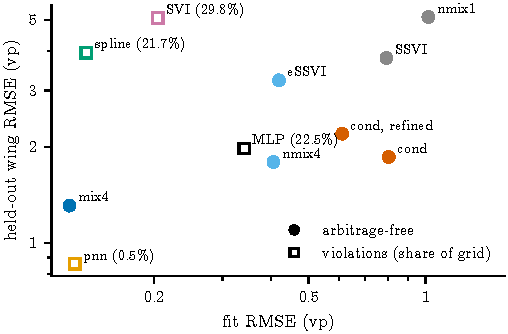
\includegraphics[width=0.6\linewidth]{tradeoff.pdf}
  \caption{Fit against wing extrapolation on SPX 2022 (both log scales). Filled markers are
  arbitrage-free on the whole widened grid; open markers violate it, with the calendar plus
  butterfly violation share in parentheses.}
  \label{fig:tradeoff}
\end{figure}

\subsection{Test year and replication window}

\Cref{tab:oos} reports the same metrics on SPX 2023 and on 2016--2017. On 2023 only the mixture and
the conditional models were scored. The mixture again fits closest (\mixFitTest\vp). The conditional
model trained on 2010--2021 and refitted before each quarter is the best on the wings
(\condWingTest{} against \mixWingTest\vp). That run was the third on 2023, and the wing gain is
uneven: the refitted model is better on only 27 of the 50 days. On 2016--2017, which no choice was
tuned on, every model was scored once with the settings chosen on 2022. The rankings of 2022 hold:
the mixture fits closest and is arbitrage-free (\mixFitRep\vp, \mixInRep{} inside the bid-ask), the
penalized network has the best wings (\pnnWingRep\vp) with a few violations left, and SVI and the
spline violate the calendar condition. One 2023 finding does not replicate: the walk-forward
conditional model trails the mixture on the wings (\condWingRep{} against \mixWingRep\vp). Every
model sits inside the bid-ask more often than in 2022, because spreads were wider (median
half-spreads of 0.14--0.20 against 0.10\vp).

\begin{table}[t]
  \centering\small
  \caption{Surface models on the test year and on the replication window; columns as in
  \cref{tab:models}. On 2023 only the mixture and the conditional models were scored. ``Frozen''
  models stop training at the end of their training years; ``walk-forward'' copies are fine-tuned
  before each quarter on every day up to its start.}
  \label{tab:oos}
  \begin{tabular}{lrrrrrrr}
\toprule
& \multicolumn{4}{c}{quotes (RMSE in vp)} & \multicolumn{2}{c}{violations} & \\
\cmidrule(lr){2-5}\cmidrule(lr){6-7}
model & fit & in spread & strikes & wings & calendar & butterfly & s/day \\
\midrule
\multicolumn{8}{l}{\emph{SPX 2023, test year (50 days)}} \\
eSSVI mixture (\texttt{mix4}) & $\mathbf{0.071}$ & \textbf{80\%} & $\mathbf{0.076}$ & $0.82$ & 0 & 0 & $26$ \\
conditional, 2018--2021, frozen & $0.610$ & 13\% & $0.611$ & $1.44$ & 0 & 0 & $0.05$ \\
conditional, 2018--2021, walk-forward & $0.397$ & 20\% & $0.397$ & $0.85$ & 0 & 0 & $0.05$ \\
conditional, 2010--2021, frozen & $0.476$ & 17\% & $0.478$ & $1.25$ & 0 & 0 & $0.08$ \\
conditional, 2010--2021, walk-forward & $0.376$ & 19\% & $0.377$ & $\mathbf{0.70}$ & 0 & 0 & $0.08$ \\
\quad the same, refined & $0.323$ & 25\% & $0.324$ & $0.78$ & 0 & 0 & $1.90$ \\
\midrule
\multicolumn{8}{l}{\emph{SPX 2016--2017, replication (101 days)}} \\
SSVI & $0.614$ & 37\% & $0.622$ & $1.83$ & 0 & 0 & $0.12$ \\
SVI (per slice) & $0.128$ & 90\% & $0.138$ & $2.67$ & 15.64\% & 10.92\% & $8.39$ \\
smoothing spline & $0.130$ & 83\% & $0.147$ & $2.23$ & 7.43\% & 0.66\% & $<0.01$ \\
penalized network (\texttt{pnn}) & $0.085$ & 96\% & $0.086$ & $\mathbf{0.32}$ & 0.08\% & 0.00\% & $194$ \\
eSSVI mixture (\texttt{mix4}) & $\mathbf{0.068}$ & \textbf{99\%} & $\mathbf{0.071}$ & $0.35$ & 0 & 0 & $32$ \\
conditional, 2010--2015, frozen & $0.512$ & 34\% & $0.507$ & $0.75$ & 0 & 0 & $0.11$ \\
conditional, 2010--2015, walk-forward & $0.375$ & 43\% & $0.373$ & $0.55$ & 0 & 0 & $0.07$ \\
\quad the same, refined & $0.289$ & 55\% & $0.288$ & $0.52$ & 0 & 0 & $1.56$ \\
\bottomrule
\end{tabular}

\end{table}

\subsection{Regime change limits the cross-day model on SPX}

On SPX 2022 the conditional model fits five to seven times worse than the mixture
(\cref{tab:models}), because 2022 left the family of surfaces it learned. Its amortized error is
\condQIn--\condQInMax\vp{} in every sampled quarter of 2019 and 2021, but \condQOne\vp{} in 2022Q1 and
\condQFour\vp{} by 2022Q4, while the ATM skew $\partial\sigma/\partial k$ flattens from $\skewQOne$
to $\skewQFour$ (\cref{fig:regime}). Neither the encoder nor the maturity grid is the cause:
thinning the extra short-dated expiries of 2022 back to the training count leaves the error
unchanged, the mixture restricted to the decoder's maturity grid still fits 2022 to 0.19--0.29\vp,
and refining the latent recovers only 3--11\% of the error. Walk-forward refits close about half of
the 2022 gap, and training from 2010 lowers the error everywhere (\cref{tab:oos}), but the frozen
model's 2022 error stays twice its early-stopping error, so 2022 also lies outside 2010--2021.

\begin{figure}[t]
  \centering
  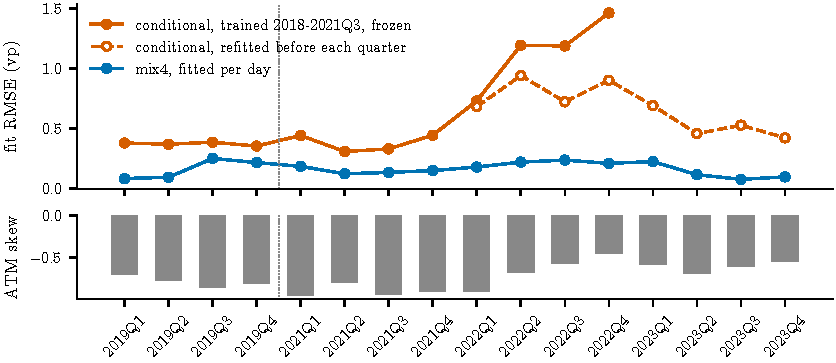
\includegraphics[width=\linewidth]{regime.pdf}
  \caption{Amortized fit error of the conditional model by quarter on the evaluation days, frozen
  after training on 2018--2021Q3 and refitted before each quarter, against the per-day mixture; the
  lower panel is the quarter's ATM skew $\partial\sigma/\partial k$. 2020 was not sampled (dotted line).}
  \label{fig:regime}
\end{figure}

\subsection{Missing strikes and maturities}

\Cref{fig:gaps} refits every model with more of each chain held out. On SPX the per-day mixture
degrades slowly and stays best: with 90\% of interior strikes held out it misses them by
\mixGapNinety\vp, against \sviGapNinety{} for SVI and \condGapNinety{} for the refined conditional
model. With 30\% of inner maturities held out it misses by \mixGapSlices\vp, against \condGapSlices{}
for the conditional model and \sviGapSlices{} for SVI, which also violates calendar arbitrage there.
The conditional model's error barely moves with the share held out, on both panels, and on Heston it
is best at every level: with 90\% of strikes missing its error against the true surface is
\hestonTruthNinetyCond\vp, against \hestonTruthNinetyMix{} for the mixture. At 90\% SVI cannot fit any
Heston day, because too few strikes remain per slice.

\begin{figure}[t]
  \centering
  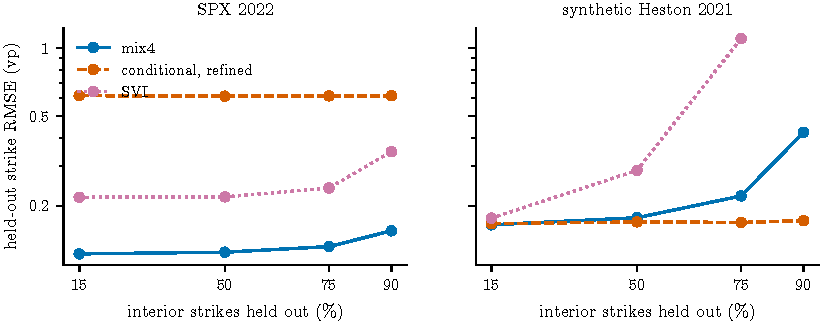
\includegraphics[width=\linewidth]{gaps.pdf}
  \caption{Error on held-out interior strikes as more of each chain is held out (log scale); every
  model is refitted at each level. SVI cannot fit a Heston day with 90\% held out.}
  \label{fig:gaps}
\end{figure}

\subsection{Synthetic panels: the cross-day model wins}

On synthetic Heston, whose regime does not change between years, the cross-day model is the best
surface model (\cref{tab:heston}). Trained on one year, it already beats the mixture against the
truth on the validation year, but its amortized error rises by 70--80\% on the test years, whose
variance falls below anything in its training year. Trained on nine generator years, it is less than half as far from
the true surface as the mixture on every panel, with the closest wings and \multiInFresh{} of its
model IVs inside the bid-ask, in an \multiTime\,ms forward pass against \mixTimeHeston\,s. The
mixture stays closest to the quotes themselves, because it also fits each day's quote noise.

\begin{table}[t]
  \centering\small
  \caption{Error against the true surface on synthetic Heston (vp): held-out interior strikes and
  held-out wings, on the validation year, the test year and a fresh test panel generated with a new
  seed. The conditional model is trained on one year (2020) or on nine.}
  \label{tab:heston}
  \begin{tabular}{lrrrrrr}
\toprule
& \multicolumn{3}{c}{held-out strikes} & \multicolumn{3}{c}{held-out wings} \\
\cmidrule(lr){2-4}\cmidrule(lr){5-7}
model & 2021 (val.) & 2022 (test) & fresh 2023 & 2021 & 2022 & fresh 2023 \\
\midrule
eSSVI mixture (\texttt{mix4}) & $0.094$ & $0.098$ & $0.099$ & $0.248$ & $0.254$ & $0.244$ \\
conditional, one year & $0.083$ & $0.138$ & $0.152$ & $0.138$ & $0.187$ & $0.222$ \\
\quad refined & $0.062$ & $0.078$ & $0.082$ & $0.145$ & $0.159$ & $0.173$ \\
conditional, nine years & $0.040$ & $0.045$ & $0.045$ & $\mathbf{0.112}$ & $\mathbf{0.109}$ & $\mathbf{0.127}$ \\
\quad refined & $\mathbf{0.040}$ & $\mathbf{0.040}$ & $\mathbf{0.042}$ & $0.128$ & $0.120$ & $0.135$ \\
\bottomrule
\end{tabular}

\end{table}

\subsection{Forecasting}

No model forecasts the surface better than a random walk (\cref{tab:forecast} in
\cref{app:forecast}). On SPX the latent
VAR loses to the origin day's mixture surface at one day ($p<0.001$), because the decoded surface's
own 2022 error (last column) is almost as large as a one-day move. At 20 days its error is lower
(\fcVarTwenty{} against \fcRwTwenty\vp), but not significantly ($p=\fcPTwenty$). The Heston panel is
the positive control. The latent encodes the true log-variance almost linearly (out-of-sample
$R^2=0.995$), and forecasting that state with the generator's own dynamics beats the random walk by
24\% at 20 days ($p=0.03$). An AR(1) fitted to the true state over the single training year, however,
loses by 80\%, and the latent VAR by a similar margin: one year of a process with a 35-day half-life
is too short to estimate its mean. The representation carries the forecastable signal, but its
dynamics cannot be estimated from one year.

\section{Mispricing detection}
\label{sec:mispricing}

\subsection{Detectors}

A least-squares fit absorbs part of every mispriced quote into the surface. Each detector therefore
refits the day's \mixfour{} surface by iteratively reweighted least squares~\citep{holland1977} for a
Cauchy loss on residuals in half-spreads: a quote $u$ half-spreads from the surface has its
half-spread widened by $\sqrt{1+(u/c)^2}$, and the surface is refitted from the previous pass
(\cref{app:robust}). The traded detector, robust \mixfour, uses scale $c=1$ and two passes. A
mispriced segment of neighbouring strikes survives this refit, because each quote's weight reads
only its own residual and a smooth bump leaves each one small. The pooled robust detector therefore
weights each quote by the larger of its own residual and the mean residual over up to two strikes on
either side in its expiry ($c=0.25$, 16 passes), which down-weights a run of same-signed residuals as
a whole. It was chosen among 24 settings on Heston 2021 by the highest recall among settings at least
as precise as robust \mixfour. On the synthetic panels the cross-day model is a third detector: its
surface moves only through the latent, so it absorbs almost none of a mispricing.

Residuals are signed so that positive means the market is rich. A quote is flagged when the model
price lies outside the bid-ask by more than a margin $m$, in price half-spreads: rich quotes are sold
and cheap ones bought. Margins were chosen on the validation years: $m=0.5$ on synthetic data and
$m=4$ on SPX, where the conditional model is not used because its error is several times the
half-spread.

\subsection{Synthetic panels}

\Cref{tab:detection,fig:detection} score the detectors against the injected labels. Least-squares
fits absorb about half of a mispriced segment into the surface, and the robust refit barely changes
that (\robAbsorbFresh{} on the fresh panel); pooling cuts it to \segAbsorbFresh, and at the robust
detector's precision it adds 9 points of recall and 14 of segment recall. The conditional model
trained on nine years is the best detector on both test panels: precision \multiPrecFresh{} at recall
\multiRecFresh{} on the fresh panel, with \multiSegFresh{} of mispriced segments found, against
\robSegFresh{} for robust \mixfour{} and \segSegFresh{} for the pooled refit. Its precision is
0.995--0.998 in every quarter. The one-year model has the same recall but loses precision in two
quarters of each panel (0.35--0.52), where the variance leaves the range of its training year; in
2022Q4 its error against the true surface triples. Flagged residuals of the nine-year detector revert by
$-0.52$, $-0.95$ and $-0.99$ at 1, 3 and 5 days on Heston 2022, against an injected decay of $-0.50$,
$-0.875$ and $-0.97$.

\begin{table}[t]
  \centering\small
  \caption{Detection at margin 0.5 on the synthetic test panels, Heston 2022 / fresh panel. Labels are
  injected shifts above one half-spread; recall is split into isolated strikes and segments, and
  ``absorbed'' is the median share of a mispriced segment the detector's surface absorbs.
  Best values on the fresh panel in bold.}
  \label{tab:detection}
  \begin{tabular}{lrrrrr}
\toprule
& & \multicolumn{3}{c}{recall} & \\
\cmidrule(lr){3-5}
detector & precision & recall & isolated & segments & absorbed \\
\midrule
least-squares \texttt{mix4} & $0.902$ / $0.902$ & $0.39$ / $0.40$ & $0.53$ / $0.54$ & $0.21$ / $0.23$ & 56\% / 55\% \\
robust \texttt{mix4} & $0.954$ / $0.950$ & $0.44$ / $0.45$ & $0.58$ / $0.59$ & $0.27$ / $0.29$ & 53\% / 52\% \\
pooled robust \texttt{mix4} & $0.964$ / $0.964$ & $0.52$ / $0.54$ & $0.62$ / $0.64$ & $0.40$ / $0.43$ & 36\% / 34\% \\
conditional, one year & $0.635$ / $0.581$ & $0.63$ / $0.65$ & $\mathbf{0.63}$ / $\mathbf{0.65}$ & $0.63$ / $0.65$ & 4\% / 4\% \\
conditional, nine years & $\mathbf{0.997}$ / $\mathbf{0.996}$ & $\mathbf{0.63}$ / $\mathbf{0.65}$ & $0.63$ / $0.64$ & $\mathbf{0.62}$ / $\mathbf{0.66}$ & 4\% / 3\% \\
\bottomrule
\end{tabular}

\end{table}

\begin{figure}[t]
  \centering
  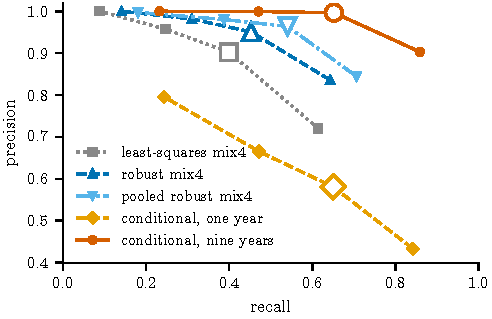
\includegraphics[width=0.54\linewidth]{detection.pdf}
  \caption{Precision against recall on the fresh synthetic panel as the margin falls from 2 to 0
  half-spreads; open circles mark the chosen margin 0.5.}
  \label{fig:detection}
\end{figure}

\subsection{Fitting failures and refits}
\label{sec:refits}

The first SPX runs used cached least-squares fits from the default start, and on some days that
start stops in a poor local minimum, in which the surface misses whole expiries. Such a day flags
many quotes that are not mispriced. The problem surfaced on 2016--2017, where 92\% of the cached-fit
flags fell on four days of October 2017. Every mispricing panel was therefore refitted: each day's
least-squares surface is the better, by its own objective, of the cached fit and a fit started from
the previous day's chosen surface, so days are fitted in date order, and the robust refits start
from it. This rule and every other setting were frozen on the validation years, together with a
written prediction of the outcome, before the test panels were run once more.

\Cref{tab:refit,fig:refit} show how often the cached fits failed. On \refitTwoX{} of the
\refitDays{} days of SPX 2023 the cached objective was more than twice what the surface can reach
(median ratio \refitMedian), and on the worst day of 2017 it was a hundred times higher. Validation
2022 and 2016 had milder failures, and the synthetic panels, drawn from one smooth model, had none.
On the validation years the refits changed little: the backtest selection rule again picked the
same margin and holding period, and the synthetic detection table is all but unchanged, so every
other setting was kept. The surface comparisons of \cref{sec:surfaces} fit \mixfour{} on their own
sampled days and were not rerun; minima there would overstate the mixture's fit error.

\begin{table}[t]
  \centering\small
  \caption{Least-squares objective of the chosen fit relative to the cached fit, per panel: days on
  which the previous-day start won, the median ratio, days with an objective more than 10\% and more
  than twice lower, and the worst day's objectives (mean squared IV residual in half-spreads).}
  \label{tab:refit}
  \begin{tabular}{lrrrrl}
\toprule
& & & \multicolumn{2}{c}{days lower by} & \\
\cmidrule(lr){4-5}
panel & start won & median & $>10\%$ & $>2\times$ & worst day \\
\midrule
SPX 2022 (validation) & 154 / 253 & $0.97$ & 54 & 0 & 0.47 $\to$ 0.25 (Sep 9) \\
SPX 2023 (test) & 205 / 247 & $0.69$ & 172 & 69 & 0.53 $\to$ 0.12 (Jul 7) \\
SPX 2016 & 105 / 251 & $1.00$ & 20 & 0 & 0.15 $\to$ 0.12 (Oct 27) \\
SPX 2017 & 144 / 250 & $0.96$ & 83 & 12 & 5.51 $\to$ 0.05 (Oct 24) \\
Heston 2021 & 41 / 261 & $1.00$ & 0 & 0 & -- \\
Heston 2022 & 48 / 234 & $1.00$ & 0 & 0 & -- \\
Heston, fresh 2023 & 42 / 260 & $1.00$ & 0 & 0 & -- \\
\bottomrule
\end{tabular}

\end{table}

\begin{figure}[t]
  \centering
  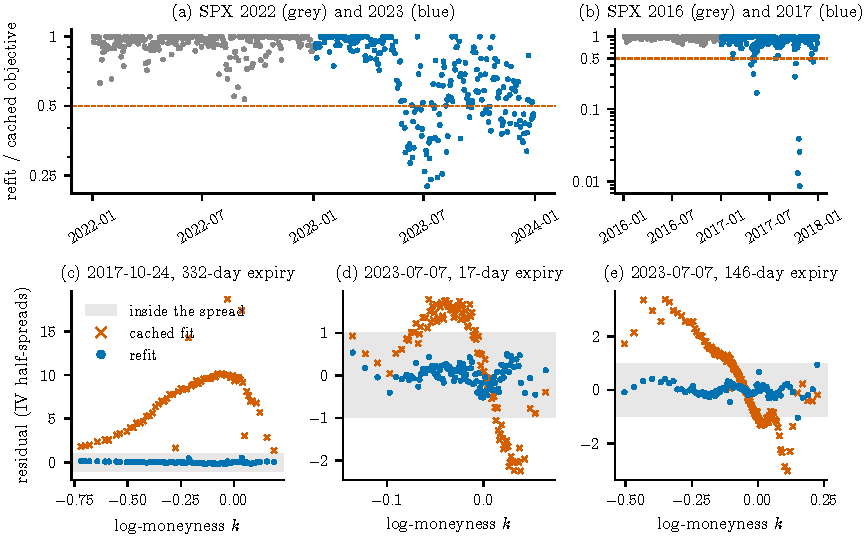
\includegraphics[width=\linewidth]{refit.pdf}
  \caption{(a, b) Refit-to-cached objective ratio per day (log scale); below the dashed line the
  cached fit was more than twice the reachable objective. (c--e) Residuals in IV half-spreads of the
  cached fit and the refit on (c) the SPX day with the largest reduction, October 24, 2017, at its
  expiry with the largest cached-fit error, and (d, e) the worst day of 2023 at its two such
  expiries; the shaded band is inside the spread.}
  \label{fig:refit}
\end{figure}

\subsection{Do flagged residuals revert?}

For each origin day and horizon $h$, the residual change of every contract quoted on both days is
regressed on its residual, separately for flagged and unflagged quotes; the daily slopes are averaged
and tested with Newey--West errors~\citep{fama1973,newey1987} (\cref{app:reversion}). A slope of
$-1$ is full reversion within $h$ days. Quote noise makes residuals revert even where nothing is
mispriced, so unflagged quotes are the control.

On the cached fits of SPX 2023, flagged residuals reverted faster than unflagged ones at every horizon
(\cref{tab:reversion}; $\revCachedDiffOne$ at one day, $p=\revCachedPOne$, on \revCachedDays{} days with at
least five flags). On the refits the robust detector flags 0.30\% of quotes (0.44\% before), with at
least five flags on \revDays{} days, and the one-day difference vanishes ($\revDiffOne$,
$p=\revPOne$). At 3 and 5 days a difference remains. The pooled detector's flags still revert faster
than unflagged ones at every horizon ($p<0.001$, \revSegDays{} days).

Reversion of a residual can come from either side: the market quote can move towards the surface,
or the surface, refitted each day, can move towards the quote. Only the first is a mispricing that
can be traded. With $x_t=(\sigma^{\text{mkt}}_t-\sigma^{\text{model}}_t)/s_t$ and $s_t$ the origin
day's IV half-spread, the slope of $x_{t+h}-x_t$ on $x_t$ splits exactly into the slope of the market
part minus that of the model part (\cref{app:reversion}). The lower block of \cref{tab:reversion}
shows the split. Neither detector's flagged prices move towards the model more than unflagged prices
do at one day ($p=\revMarketPOne$ for the robust detector). At 3 and 5 days the pooled detector's
flags revert mostly through the surface moving, and its flagged prices move significantly
\emph{less} towards the model than unflagged ones: distinguishable, but in the direction against a
tradable mispricing.

\begin{table}[t]
  \centering\small
  \caption{Reversion on SPX 2023 at margin 4. Upper block: flagged minus unflagged reversion slope of
  price residuals ($p$-values in parentheses; negative means flags revert faster). Lower block: slopes
  of IV residuals in origin-day half-spreads, split into the market's move and the model's; a
  positive model part is the surface moving towards the quote. The last rows test whether flagged
  prices move towards the model more than unflagged ones.}
  \label{tab:reversion}
  \begin{tabular}{lrrr}
\toprule
 & 1 day & 3 days & 5 days \\
\midrule
\multicolumn{4}{l}{\emph{reversion slope, price residuals, robust \texttt{mix4}}} \\
cached fits, flagged $-$ unflagged & $-0.23$ ($0.002$) & $-0.23$ ($<0.001$) & $-0.18$ ($0.003$) \\
refits, flagged $-$ unflagged & $-0.05$ ($0.72$) & $-0.24$ ($0.006$) & $-0.17$ ($0.05$) \\
\midrule
\multicolumn{4}{l}{\emph{IV residuals split into market and model moves (refits)}} \\
robust: flagged, market part & $-0.28$ ($0.17$) & $-0.53$ ($0.12$) & $-0.93$ ($0.02$) \\
robust: flagged, model part & $+0.01$ & $-0.04$ & $-0.57$ \\
robust: unflagged, market part & $-0.34$ & $-0.59$ & $-0.74$ \\
robust: market, flagged $-$ unflagged ($p$) & $0.89$ & $0.36$ & $0.72$ \\
pooled robust: flagged, market part & $-0.19$ ($0.13$) & $-0.08$ ($0.65$) & $-0.21$ ($0.36$) \\
pooled robust: flagged, model part & $+0.14$ & $+0.40$ & $+0.41$ \\
pooled robust: unflagged, market part & $-0.33$ & $-0.70$ & $-1.10$ \\
pooled robust: market, flagged $-$ unflagged ($p$) & $0.39$ & $<0.001$ & $<0.001$ \\
\bottomrule
\end{tabular}

\end{table}

\paragraph{The written prediction.} Before the test run we predicted that (i) the next-day reversion
of flags would mostly not be the market moving, and (ii) the flagged market move would not be
distinguishable from the unflagged one. Part (i) was not borne out at one day: most of the flagged
residuals' one-day change is the market's (robust $-0.28$ of $-0.29$; pooled $-0.19$ of $-0.33$),
though neither part is significant. At 3 and 5 days it holds for the pooled detector. Part (ii) holds
for robust \mixfour{} at every horizon and for the pooled detector at one day; at 3 and 5 days the
pooled detector's flagged prices are distinguishable, but they move less towards the model.

\subsection{Backtest}

Each flag of the traded detector is traded with \$1{,}000 of vega, crossing the spread on entry and
exit and paying \$1 per contract per side. It is delta-hedged daily with its expiry's forward and
closed once its residual is below half a spread, or after five days (\cref{app:backtest}). Next-day
execution, with the signal at one close and the trade at the next, is the main case; same-day
execution is an optimistic bound, since it assumes a fill at the closing quotes that produced the
signal. Each trade has 20 placebos: random unflagged contracts from the same day, type, direction and
maturity--moneyness bucket, held for the same days. The placebos earn what the strategy's exposure
earns, such as the volatility risk premium on sold options~\citep{bakshi2003,carr2009}, without its
signal.

\begin{table}[t]
  \centering\small
  \caption{Delta-hedged backtest of the traded detector at margin 4, holding at most five days, with
  20 matched placebos per trade. Sharpe ratios are annualized from daily net PnL; ``placebo'' is the
  placebos' mean net and ``excess'' the strategy's net minus it, with a Newey--West $p$-value. The validation row
  is the cell chosen by the selection rule, so it is biased upward. The synthetic rows trade the
  one-year conditional detector; trading the true labels checks the accounting.}
  \label{tab:backtest}
  \begin{tabular}{lrrrrrrr}
\toprule
execution & trades & gross & costs & net & Sharpe & placebo & excess ($p$) \\
\midrule
\multicolumn{8}{l}{\emph{SPX 2023 test, refits}} \\
next day & 1{,}482 & $+$\$476k & \$184k & $+$\$292k & $0.99$ & $+$\$233k & $+$\$59k ($0.31$) \\
same day (bound) & 1{,}586 & $+$\$545k & \$176k & $+$\$368k & $1.63$ & $+$\$48k & $+$\$320k ($0.02$) \\
\midrule
\multicolumn{8}{l}{\emph{SPX 2023 test, cached fits}} \\
next day & 2{,}595 & $+$\$162k & \$354k & $-$\$192k & $-0.66$ & $-$\$292k & $+$\$100k ($0.09$) \\
same day (bound) & 2{,}883 & $+$\$421k & \$351k & $+$\$70k & $0.35$ & $-$\$353k & $+$\$423k ($0.002$) \\
\midrule
\multicolumn{8}{l}{\emph{SPX 2022 validation, refits}} \\
next day & 3{,}420 & $+$\$948k & \$771k & $+$\$178k & $0.14$ & $-$\$454k & $+$\$632k ($0.02$) \\
\midrule
\multicolumn{8}{l}{\emph{SPX 2016--2017 replication, refits}} \\
next day & 3 & $+$\$2 & \$2.2k & $-$\$2.2k & $-1.03$ & $-$\$1.4k & $-$\$781 ($0.45$) \\
same day (bound) & 4 & $-$\$2.7k & \$1.9k & $-$\$4.5k & $-1.06$ & $-$\$3.8k & $-$\$741 ($0.51$) \\
\midrule
\multicolumn{8}{l}{\emph{Heston 2022 test, conditional (one year)}} \\
next day & 3{,}091 & $+$\$998k & \$1.58m & $-$\$584k & $-5.39$ & $-$\$1.52m & $+$\$940k ($<0.001$) \\
same day (bound) & 3{,}329 & $+$\$2.12m & \$1.74m & $+$\$383k & $3.09$ & $-$\$1.69m & $+$\$2.07m ($<0.001$) \\
true labels, same day & 2{,}786 & $+$\$1.75m & \$1.54m & $+$\$206k & $1.92$ & $-$\$1.55m & $+$\$1.75m ($<0.001$) \\
\bottomrule
\end{tabular}

\end{table}

\Cref{tab:backtest} gives the results. The accounting passes its check: trading the true synthetic
labels at the signal's close makes money net of costs. On the refitted SPX 2023 panel the next-day
strategy nets \btNet{} (\btTrades{} trades, Sharpe \btSharpe), but placebos net \btPlacebo{} over the
same holding days, and the excess, \btExcess, is not significant ($p=\btP$). \btSold{} of the trades are
sales in a year in which implied volatility fell, so the profit is likely the volatility risk
premium. The same-day bound beats its placebos ($p=\btSameP$), which does not contradict the slope
test. Placebos are contracts with small residuals, whereas a flag sits at least four half-spreads
outside the bid-ask: if it reverts by the same fraction as an unflagged quote, it still moves several
times as many dollars. The slope test asks whether it reverts by a larger fraction, and at one day it
does not. On the cached fits the next-day strategy lost \btCachedNet{}, with an edge over placebos
that was not significant either ($p=\btCachedP$).

On 2016--2017 the refits leave almost nothing to flag. Spreads are wider and the mixture sits inside
them, so margin 4 is a two to three times larger deviation in vol points than in 2023: the robust
detector flags 0.003\% of quotes, at most two days have five flags, and the strategy makes
\btRepTrades{} trades. Unflagged residuals there revert by $-0.79$, $-0.85$ and $-0.88$ at 1, 3 and
5 days, against $-0.33$, $-0.45$ and $-0.51$ in 2023, closer to the synthetic panels, which suggests
that residuals inside the spread are mostly quote noise rather than persistent misfit.

\section{Limitations}
\label{sec:limitations}

\begin{itemize}
  \item \textbf{Test windows were reused.} SPX 2023 was run four times, Heston 2022 three times, and
  the fresh Heston panel and SPX 2016--2017 twice each (\cref{tab:windows}). Each later run was frozen
  on the validation years first, and the last SPX run was preceded by a prediction written before
  its test panels were fitted (\cref{app:prediction}; its configurations were committed as
  \texttt{30c766c}), but a finding on a test window chose which question the next run asked. Any further change to the
  detector has to be chosen on the validation years. SPX 2016--2017 is the only window on which the
  surface comparison was run once, and it reproduces the 2022 and 2023 rankings.
  \item \textbf{The validation backtest is biased upward.} Its row is the best of 12 cells (margin
  and holding period) it was selected from.
  \item \textbf{End-of-day data make fills optimistic.} Every trade assumes a fill at the closing
  bid or ask, with no market impact. Even the same-day bound assumes a fill at the closing quotes
  that produced the signal. Intraday quotes would be needed to test whether any of the same-day edge
  is reachable.
  \item \textbf{The surface comparisons were not refitted.} \Cref{sec:surfaces} fits \mixfour{} on its
  own sampled days from the default start, before the local minima of \cref{sec:refits} were found.
  A poor minimum raises a day's fit error, so the mixture's lead in fit is, if anything,
  understated; its held-out and wing errors could move either way.
  \item \textbf{Sufficient conditions cost extrapolation.} The eSSVI conditions are sufficient
  rather than necessary, and they bind at the fitted knots on SPX. Arbitrage-free wings closer to the
  penalized network's would need a richer feasible family.
  \item \textbf{The cross-day model is only as good as its training regimes.} On SPX the market
  moved outside them in 2022, and quarterly refits close only part of the gap. On the synthetic
  panels the latent carries the forecastable state, but a linear model fitted to one year cannot
  estimate its dynamics; nonlinear dynamics models were not tried.
  \item \textbf{The synthetic panels come from one smooth model.} The detection results depend on
  the injected mispricings' form and on a stationary regime, and the per-day minima that broke the
  SPX fits do not occur there. They show what the detectors can find, not what SPX contains.
  \item \textbf{Platforms.} The validation panels were fitted on macOS (arm64) and the last test
  panels on Linux (x86-64) with the same Python and locked dependencies. Six SPX 2022 days fitted
  both ways agree to rounding; the conditional detectors' per-day refinement differs by at most
  0.034\vp{} a quote, which changes 4 of 7{,}480 flags on Heston 2022.
\end{itemize}

\section{Conclusion}
\label{sec:conclusion}

A price-space mixture of four eSSVI surfaces, arbitrage-free for every parameter vector, is the best
per-day model of the SPX surface in every window we tested: it fits closest, it has no calendar or
butterfly violations, and it degrades slowly when strikes or maturities are missing. Penalized
networks extrapolate the wings better but keep some violations. A cross-day encoder--decoder that
decodes every latent to an arbitrage-free surface wins every task on stationary synthetic data,
including mispricing detection, but on SPX it is limited by regime change, and no model forecasts
the surface better than a random walk. Used as a reference price, the best per-day surface does not
reveal tradable SPX mispricings: once its fitting failures are removed, flagged quotes do not return
to it faster than other quotes, and a delta-hedged strategy on the flags earns what matched placebos
earn. The flags that looked like a signal on the first test run were largely the surface's own
errors.

\paragraph{Reproducibility.} The code, configurations and every Makefile target behind the tables
are in the project repository; \texttt{make figures} regenerates every figure and table of this
report from the saved results, and \texttt{make report} compiles it. The option data are licensed
from OptionsDX and are not redistributed; the synthetic panels are regenerated with
\texttt{make synthetic}.


\bibliographystyle{plainnat}
\bibliography{refs}

\appendix
\section{Static arbitrage in total variance}
\label{app:arbitrage}

Fix a maturity $T$ with forward $F$ and discount factor $D$, and write the call price as
$C(K)=DF\,c(k)$ with $k=\log(K/F)$ and $c(k)=c_{\text{B}}\bigl(k,w(k)\bigr)$, where
\[
  c_{\text{B}}(k,w)=N(d_1)-e^{k}N(d_2),\qquad d_{1,2}=-\frac{k}{\sqrt w}\pm\frac{\sqrt w}{2}.
\]
Black's partial derivatives are $\partial_k c_{\text{B}}=-e^kN(d_2)$,
$\partial_w c_{\text{B}}=e^k\phi(d_2)/(2\sqrt w)>0$ and
$\partial_{kk}c_{\text{B}}-\partial_k c_{\text{B}}=e^k\phi(d_2)/\sqrt w=2\,\partial_w c_{\text{B}}$, using
$\phi(d_1)=e^k\phi(d_2)$.

\paragraph{Calendar.} With deterministic rates and proportional dividends, a calendar spread at a
fixed forward-moneyness is free of arbitrage if and only if $c(k,T)$ is nondecreasing in $T$ at fixed
$k$~\citep{carr2005,gatheral2014}. Since $\partial_w c_{\text{B}}>0$, this holds if and only if
$\partial_T w(k,T)\ge 0$.

\paragraph{Butterfly.} The risk-neutral density of the underlying at $T$ is
$q(K)=D^{-1}\partial^2_K C$~\citep{breeden1978}. Since $\partial_K=K^{-1}\partial_k$,
$\partial^2_K C=DF K^{-2}(c''-c')$, with primes the total derivatives in $k$. Expanding $c'$ and $c''$
through $w(k)$,
\[
  c''-c'=(\partial_{kk}-\partial_k)c_{\text{B}}+(2\partial_{kw}-\partial_w)c_{\text{B}}\,w'
  +\partial_{ww}c_{\text{B}}\,w'^2+\partial_w c_{\text{B}}\,w''.
\]
Differentiating $\partial_w c_{\text{B}}$ gives $\partial_{kw}c_{\text{B}}=\partial_w c_{\text{B}}\,(1+d_2/\sqrt w)$ and
$\partial_{ww}c_{\text{B}}=\partial_w c_{\text{B}}\,\bigl(k^2/(2w^2)-1/(2w)-1/8\bigr)$. Substituting
$d_2/\sqrt w=-k/w-1/2$ and collecting terms,
\[
  c''-c'=2\,\partial_w c_{\text{B}}\Bigl[1-\frac{kw'}{w}+\Bigl(\frac{k^2}{4w^2}-\frac{1}{4w}-\frac1{16}\Bigr)w'^2+\frac{w''}{2}\Bigr]
  =2\,\partial_w c_{\text{B}}\;g(k),
\]
with $g$ as in \cref{eq:conditions}. Hence $q(K)=\phi\bigl(d_2(k)\bigr)\,g(k)/\bigl(K\sqrt{w(k)}\bigr)$,
which is nonnegative exactly where $g$ is~\citep{gatheral2014}.

\paragraph{Wings.} For any arbitrage-free smile, $\limsup_{|k|\to\infty}w(k)/|k|\le2$~\citep{lee2004}.
The penalized network enforces it as a bound on the slope of $w$ at the outermost collocation
strikes; eSSVI satisfies it through $\max(u_+,u_-)<4$.

\paragraph{Grids.} Violation shares are evaluated on 40 maturities and 101 strikes per maturity (801
for the calendar check) spanning the quoted domain, and on the same grid widened by 50\% of the
quoted width on each side. A calendar violation counts when $w$ falls between consecutive grid
maturities by more than a numerical tolerance; a butterfly violation when $g<-10^{-5}$.

\section{eSSVI parametrization and price mixtures}
\label{app:essvi}

\paragraph{Feasible knots.} At knot maturities $T_1<\dots<T_n$, unconstrained rates
$(a_i,b_i^+,b_i^-)$ map to knots as follows, with $\operatorname{sp}$ the softplus,
$\Delta_i=T_i-T_{i-1}$ and $\delta_i=\log T_i-\log T_{i-1}$:
\[
  u^\pm_i=4\Bigl(1-\exp\Bigl(-\sum_{l\le i}\operatorname{sp}(b^\pm_l)\,\delta_l\Bigr)\Bigr),\qquad
  \theta_i=\max\Bigl(\theta_{i-1}\frac{\psi_i}{\psi_{i-1}},\;\frac{\psi_i\max(u^+_i,u^-_i)}{4}\Bigr)+\operatorname{sp}(a_i)\,\Delta_i,
\]
with $\psi_i=(u^+_i+u^-_i)/2$. The wings are nondecreasing and below 4. Because $\psi$ is
nondecreasing, $\theta_i>\theta_{i-1}$; the first term of the maximum keeps $\psi/\theta$
nonincreasing and the second is the butterfly bound $\psi\max(u_+,u_-)\le4\theta$. Every condition
of \cref{sec:models} therefore holds for every rate vector, and every feasible knot sequence with
strict increases has a preimage.

\begin{proposition}
\label{prop:mixture}
Let $c_1,\dots,c_M$ be normalized call price surfaces on a common set of expiries, each free of static
arbitrage, and let $\pi_j\ge0$ with $\sum_j\pi_j=1$ be constant in $k$ and $T$. Then
$c=\sum_j\pi_jc_j$ is free of static arbitrage, and its Black implied total variance $w(k,T)$ exists,
is unique, lies between $\min_j w_j$ and $\max_j w_j$, and satisfies \cref{eq:conditions}.
\end{proposition}

\begin{proof}
For each $T$, every $c_j$ is convex and nonincreasing in the strike and lies between
$(1-e^k)^+$ and 1; for each $k$, it is nondecreasing in $T$. Each of these properties is preserved
by a convex combination with weights that do not depend on $k$ or $T$, so $c$ has them too. Since
$w\mapsto c_{\text{B}}(k,w)$ is a strictly increasing bijection from $(0,\infty)$ onto
$\bigl((1-e^k)^+,1\bigr)$, the implied variance exists and is unique, and because $c$ lies between
$\min_j c_j$ and $\max_j c_j$ it lies between the components' variances. Monotonicity of $c$ in $T$
gives $\partial_Tw\ge0$ (\cref{app:arbitrage}). The density of $c$ is $\sum_j\pi_jq_j\ge0$, so
$g\ge0$.
\end{proof}

If the weights varied with $T$, a component with low variance could gain weight at a longer maturity
and the mixture price could fall, which is why \mixfour{} uses one set of weights per day.

\section{Forwards and discount factors from put--call parity}
\label{app:forwards}

For each expiry, take the 20 strikes nearest the forward (smallest $|C-P|$) at which both the call
and the put are quoted two-sided. Put--call parity, $C-P=DF-DK$, makes the mid price difference
linear in $K$ with slope $-D$ and intercept $DF$. The slope is weakly identified at short maturities,
where $D\approx1-rT$, so estimation runs in three stages per date: (i) a weighted regression per
expiry with $T\ge30$ days gives $r=-\log D/T$; (ii) a robust kernel smoother in $\log T$ turns these
into a rate curve, flat below 30 days; (iii) with $D=e^{-r(T)T}$ for every expiry, $F$ is the
weighted median of $K+(C-P)/D$ over the pairs. An expiry is valid when the relative median absolute
deviation of those per-strike forwards is below 0.002.

\section{Robust refits}
\label{app:robust}

The least-squares objective of a surface is $\frac1n\sum_i u_i^2$ with
$u_i=(\sigma^{\text{model}}_i-\sigma^{\text{mkt}}_i)/s_i$, where $s_i$ is the IV half-spread with a floor
of 0.1\vp. One step of iteratively reweighted least squares for the Cauchy loss
$\rho(u)=\tfrac{c^2}{2}\log\bigl(1+u^2/c^2\bigr)$ weights each quote by
$\rho'(u_i)/u_i=1/\bigl(1+u_i^2/c^2\bigr)$, the residual from the previous pass. This is the squared
loss with each half-spread replaced by $s_i\sqrt{1+u_i^2/c^2}$, so every refit reuses the
least-squares solver. The pooled variant replaces $|u_i|$ in the weight by
$\max\bigl(|u_i|,|\bar u_i|\bigr)$, where $\bar u_i$ is the mean residual of quote $i$ and up to two
strikes on either side in its expiry. Quotes that are legs of model-free arbitrage are scored but
excluded from every fit.

\section{Reversion tests}
\label{app:reversion}

For origin day $t$ and horizon $h$ (in screened trading days), let $r_{i,t}$ be the residual of
contract $i$ in price half-spreads and keep the contracts quoted on both $t$ and $t+h$. For flagged and
unflagged contracts separately, the slope $b_t$ of the cross-sectional regression
$r_{i,t+h}-r_{i,t}=a_t+b_t r_{i,t}+e_{i,t}$ is estimated on each day with at least five flags. The
reported slopes are the means of $b_t$, and the test of a difference uses the daily series
$b^{\text{flag}}_t-b^{\text{unflag}}_t$ with Newey--West standard errors~\citep{newey1987}, in the
manner of \citet{fama1973}; pooled regressions over thousands of quotes a day would overstate the
significance.

\paragraph{Decomposition.} With $x_{i,t}=(\sigma^{\text{mkt}}_{i,t}-\sigma^{\text{model}}_{i,t})/s_{i,t}$,
the change $x_{i,t+h}-x_{i,t}$ is not exactly the change of the residual, because $s$ changes between
days. Measured in the origin day's half-spread,
\[
  \frac{(\sigma^{\text{mkt}}_{i,t+h}-\sigma^{\text{model}}_{i,t+h})-(\sigma^{\text{mkt}}_{i,t}-\sigma^{\text{model}}_{i,t})}{s_{i,t}}
  =\underbrace{\frac{\sigma^{\text{mkt}}_{i,t+h}-\sigma^{\text{mkt}}_{i,t}}{s_{i,t}}}_{\text{market}}
  -\underbrace{\frac{\sigma^{\text{model}}_{i,t+h}-\sigma^{\text{model}}_{i,t}}{s_{i,t}}}_{\text{model}},
\]
and since an OLS slope is linear in the dependent variable, the slope of the left side on $x_{i,t}$ is
the market slope minus the model slope, day by day and on average. A negative market slope means
prices move towards the surface. The total in this basis differs from the price-residual slope; on
SPX 2022 the robust detector's one-day flagged slope is $-0.46$ in prices, $-0.33$ in IV and $-0.21$
in IV with the origin day's spread, so each part is compared with its own total.

\paragraph{Forecast tests.} The Diebold--Mariano statistic~\citep{diebold1995} is the mean of the
daily loss differential (baseline minus model) over its Newey--West standard error, with Bartlett
bandwidth $\max\bigl(h,\,4(n/100)^{2/9}\bigr)$ because overlapping $h$-day errors are autocorrelated
up to lag $h-1$, and a two-sided $p$-value from $t_{n-1}$.

\section{Backtest accounting}
\label{app:backtest}

A signal on day $s$ (sell if rich, buy if cheap) is executed at the close of day $s+\ell$, with
$\ell=1$ (next day) or $\ell=0$ (same day), in $n=V/(100\cdot0.01\,\nu)$ contracts, where $V=\$1{,}000$ is the
target dollar vega per vol point, 100 the contract multiplier and $\nu$ the Black vega per unit of
volatility at the signal. The
entry and the exit each cost $100\,n$ half-spreads plus \$1 per contract. Between closes $t$ and
$t+1$ a position of signed size $q=\pm100n$ earns
\[
  q\bigl[(m_{t+1}-m_t)-\Delta_t\,(F_{t+1}-F_t)\bigr],
\]
with $m$ the mid price, $\Delta_t$ the Black forward delta at the day's market IV and $F$ the expiry's
parity forward; the hedge is held in the forward. The position is closed $\ell$ days after the first
close at which its residual is below half a spread, or after five days. The panel holds
out-of-the-money options only, so an option that moves into the money is marked through parity from
the out-of-the-money option at its strike. A contract that drops out of the cleaned panel keeps its
hedge for up to three days and is marked when it is quoted again; beyond that it is closed at its
last quote. Entries are restricted to contracts that stay inside the panel until their latest
possible exit, and a contract is traded at most once at a time.

Each trade has 20 placebos, each a random unflagged and tradable contract from the signal day with
the same type, direction and maturity--moneyness bucket, entered and exited on the same days. The
strategy is compared with the mean placebo by a Newey--West test on the daily difference of net PnL.
Sharpe ratios are the mean of daily net PnL over its standard deviation, times $\sqrt{252}$.

\section{Forecasts}
\label{app:forecast}

\begin{table}[h]
  \centering\small
  \caption{Forecast RMSE (vp) on every quote of the target day, $h$ trading days ahead, on the
  validation years. RW is a random walk on the latent or on the origin day's \mixfour{} fit. The $p$-value is
  a Diebold--Mariano test~\citep{diebold1995}, with Newey--West variance~\citep{newey1987}, of the
  VAR against the \mixfour{} random walk; the last column scores the target day's own decoded surface, a floor
  for any forecast through the decoder.}
  \label{tab:forecast}
  \begin{tabular}{llrrrrr}
\toprule
panel & $h$ (days) & VAR(1) & latent RW & \texttt{mix4} RW & $p$ & decoded target \\
\midrule
SPX 2022 & $1$ & $1.73$ & $1.73$ & $\mathbf{1.35}$ & $<0.001$ & $1.19$ \\
 & $5$ & $2.70$ & $2.70$ & $\mathbf{2.53}$ & $0.15$ & $1.20$ \\
 & $20$ & $\mathbf{3.90}$ & $4.25$ & $4.27$ & $0.27$ & $1.22$ \\
Heston 2021 & $1$ & $0.64$ & $\mathbf{0.60}$ & $0.60$ & $<0.001$ & $0.20$ \\
 & $5$ & $1.30$ & $\mathbf{1.13}$ & $1.15$ & $0.03$ & $0.20$ \\
 & $20$ & $2.82$ & $\mathbf{1.93}$ & $1.96$ & $0.01$ & $0.20$ \\
\bottomrule
\end{tabular}

\end{table}

\section{The prediction written before the last test run}
\label{app:prediction}

The rule of \cref{sec:refits} was frozen on the validation years and its configurations committed
(\texttt{30c766c}) on November 2, 2026, before any test panel was refitted. The validation notes
written then, which are kept with the results rather than in the repository, ended with this
prediction for the test run, quoted verbatim:

\begin{quote}
\small\ttfamily\raggedright
PREDICTION for test: next-day residual "reversion" of flags is mostly not the market moving;
flagged market-side move not distinguishable from unflagged.
\end{quote}

\noindent The same notes recorded the validation results that motivated it: on the SPX 2022 refits
the robust detector's flags still reverted faster than unflagged ones at one day in price residuals
(difference $-0.27$), but their market part was small and not significant ($-0.10$, $p=0.62$), and
the flagged market move was not distinguishable from the unflagged one ($p=0.69$).


\end{document}
